\documentclass[../Article_Sensitivity_Analsysis.tex]{subfiles}
\graphicspath{{\subfix{../Figures/}}}
\begin{document}
	
	\subsection{Pressure}
	
	As discussed in Chapter \ref{CH:Governing_equations_chapter}, a small pressure wave propagates at the speed of sound relative to the flow. If the flow velocity is relatively low, all pressure changes are hydrodynamic (resulting from velocity motion) rather than thermodynamic. The Low Mach-number assumption leads to instant propagation of the thermodynamic pressure throughout the system. A single pressure value can be considered for the entire system, as all changes occur simultaneously throughout the machine. Figure \ref{fig:Sensitivty_P_P} illustrates a step function representing the pressure change.
	
	\begin{figure}[h!]
		\centering
		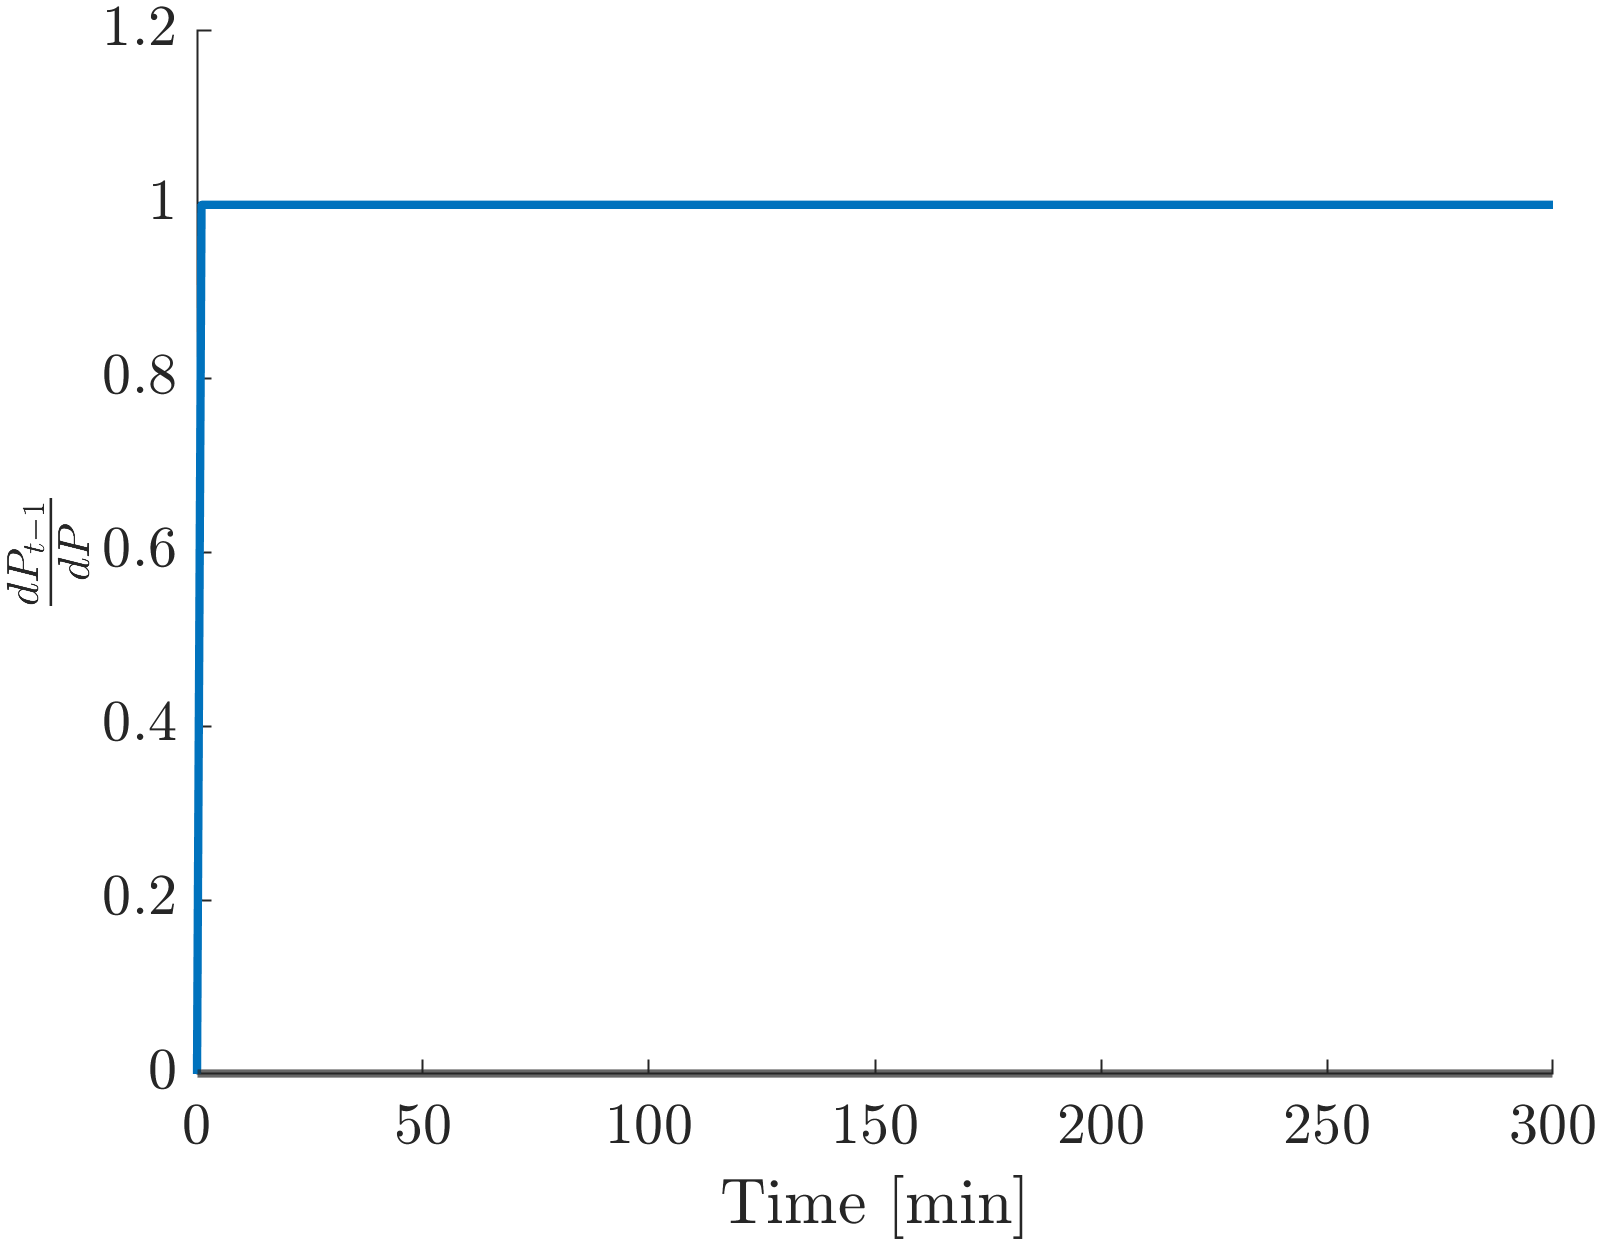
\includegraphics[trim = 0.0cm 0.0cm 0.0cm 0.0cm,clip,width=0.9\columnwidth]{/Results_sensitivity/P_P.png}
		\caption{The effect of $P$ change on $P$ in the system}
		\label{fig:Sensitivty_P_P}
	\end{figure}
	
	According to Equation \ref{EQ:Enthalpy_equation}, the pressure change directly affects the quantity $h \times \rho$ through $\frac{\partial (P(t) A_f)}{\partial t}$, leading to the step change along the whole system, as presented in Figure \ref{fig:Sensitivty_P_H}. The uniform response across the entire extraction column length and time, represented by the homogeneously dark red colour, indicates that the entire system experiences an immediate and uniform change in enthalpy density in response to pressure changes. 
	
	The pressure change influences the temperature of the fluid in the middle of the computational domain, but the values on boundaries can be defined in multiple ways. Applying the Dirichlet boundary conditions assumes a fixed temperature value at the inlet, which leads to a possible thermal gradient propagating along the system. In contrast, Neumann boundary conditions would dictate that the heat flux at the boundaries be held constant. In this work, the Neumann boundary conditions have been applied, which leads to a uniform response and ensures that the temperatures at the inlet and in the middle of the extractor are the same.
	
	\begin{figure}[h!]
		\centering
		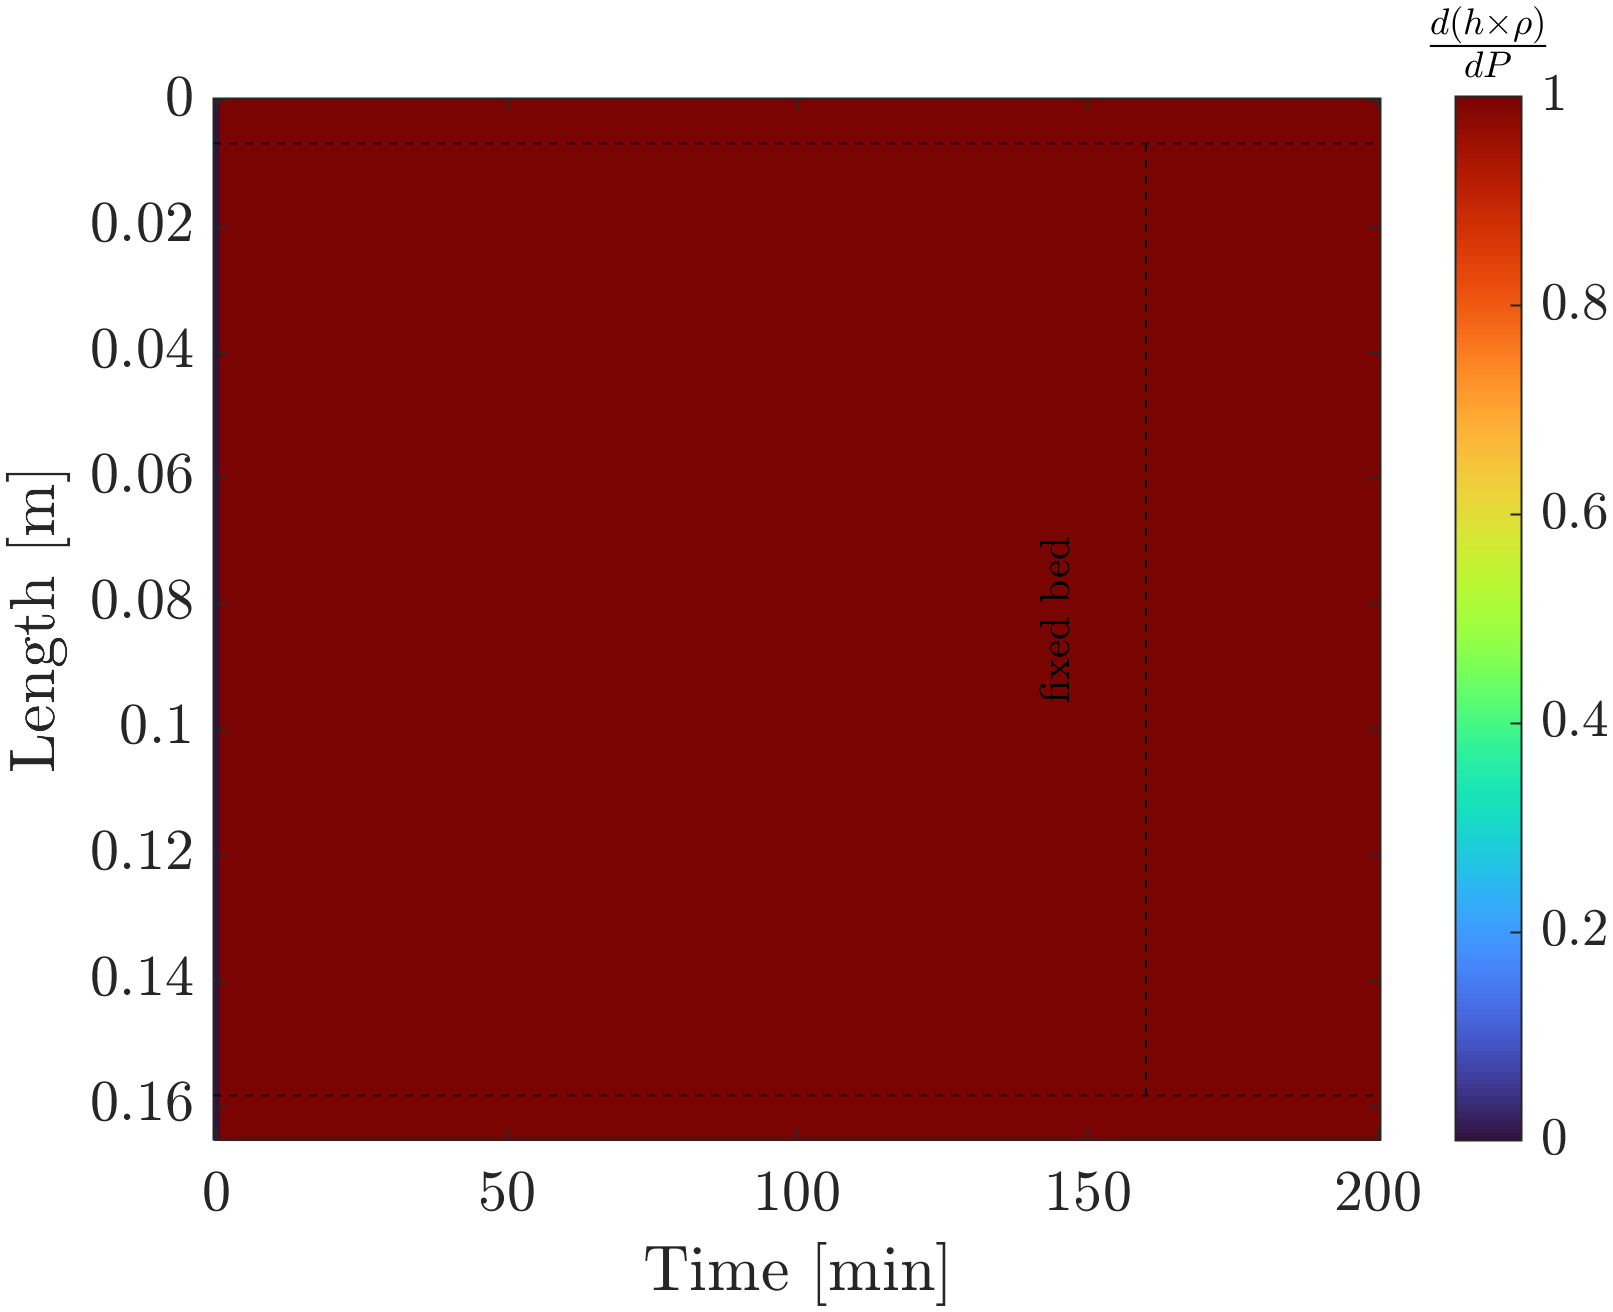
\includegraphics[trim = 0.0cm 0.0cm 0.0cm 0.0cm,clip,width=0.9\columnwidth]{/Results_sensitivity/H_P.png}
		\caption{The effect of $P$ change on $(h \times \rho)$ in the system}
		\label{fig:Sensitivty_P_H}
	\end{figure}
	
	Figure \ref{fig:Sensitivty_P_CS} shows the sensitivity of the solute concentration in the solid phase with respect to changes in pressure throughout a fixed bed in a supercritical fluid extraction process. As discussed in Chapter \ref{CH: Continuity}, the velocity of a fluid is inversely related to its density, which suggests that with higher fluid density, the velocity decreases. This leads to an extended residence time, ergo, a longer interaction between the solute and the solvent.
	
	Initially, the extraction process is in the kinetically-controlled regime, where the concentration gradient is high, and the limiting factor is the solute solubility. As explained in ({\color{red}article 1}), the system is considered to be far from the saturation, which can explain low system response at the beginning of the process. 
	
	When the concentration gradient diminishes, and the extraction moves from the kinetic-controlled to the diffusion-controlled regime, the system response becomes more profound. ({\color{red}article 1}) obtained a linear correlation for $D_i^R$, which is incorporated in this model. $D_i^R$ increases together with fluid density, which explains negative sensitivities. The negative sign can be interpreted as a faster loss of a solute from a solid phase, which corresponds to enhanced mass transfer. 
	
	Over time, the amount of solute becomes a limiting factor and the pressure change has a lower effect on the system and the sensitivities increase. Eventually, sensitivities asymptotically approach zero. The solute concentration in the solid phase has been reduced, and further changes in pressure do not influence the remaining concentration. This behaviour reflects that in the later extraction phase, the kinetics of extraction are controlled by the internal diffusion of the solute from solid particles rather than the conditions of the supercritical fluid.

	\begin{figure}[h!]
		\centering
		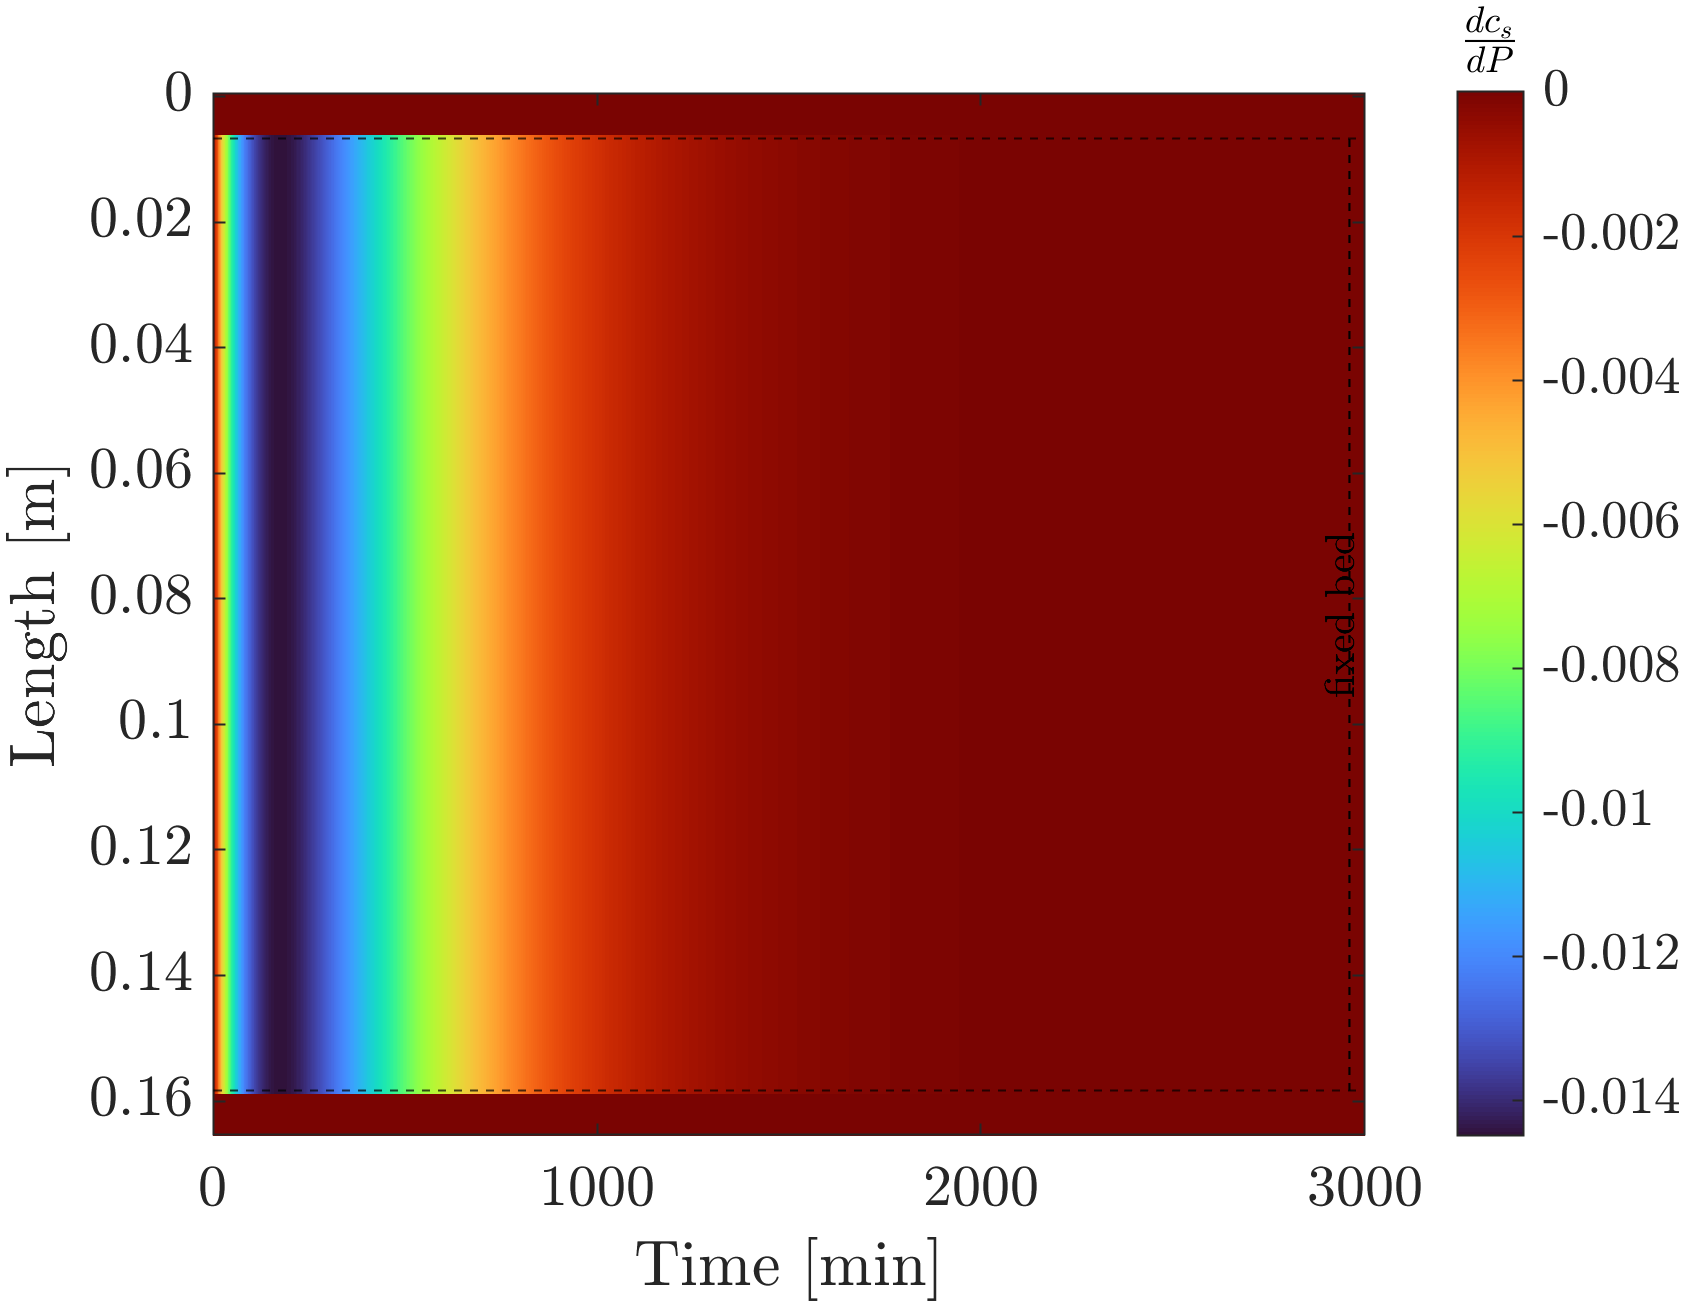
\includegraphics[trim = 0.0cm 0.0cm 0.0cm 0.0cm,clip,width=0.9\columnwidth]{/Results_sensitivity/CS_P.png}
		\caption{The effect of $P$ change on $C_s$}
		\label{fig:Sensitivty_P_CS}
	\end{figure}
	
	Figure \ref{fig:Sensitivty_P_CF} shows the sensitivity of the solute concentration in the fluid phase with respect to the pressure change. As explained above, an increase in pressure enhances the mass transfer, resulting in the concentration front moving through the system. The system response is initially low, reflecting the idle period discussed above. Later, the sensitivities increased due to enhanced mass transfer. As the fluid phase is mobile, the advection affects the sensitivities, which causes the sensitivities to move along the system analogously to the solute in the fluid phase.
	
	After the growth phase, the sensitivities start to decrease, which can be explained by the decrease in the concentration gradient. As seen in Figure \ref{fig:Sensitivty_P_CF}, sensitivities decline towards zero. This asymptotic trend suggests the driving force for the mass transfer—the concentration gradient—has been minimized, and changes in pressure no longer significantly impact the solute concentration in the fluid phase.
	
	\begin{figure}[h!]
		\centering
		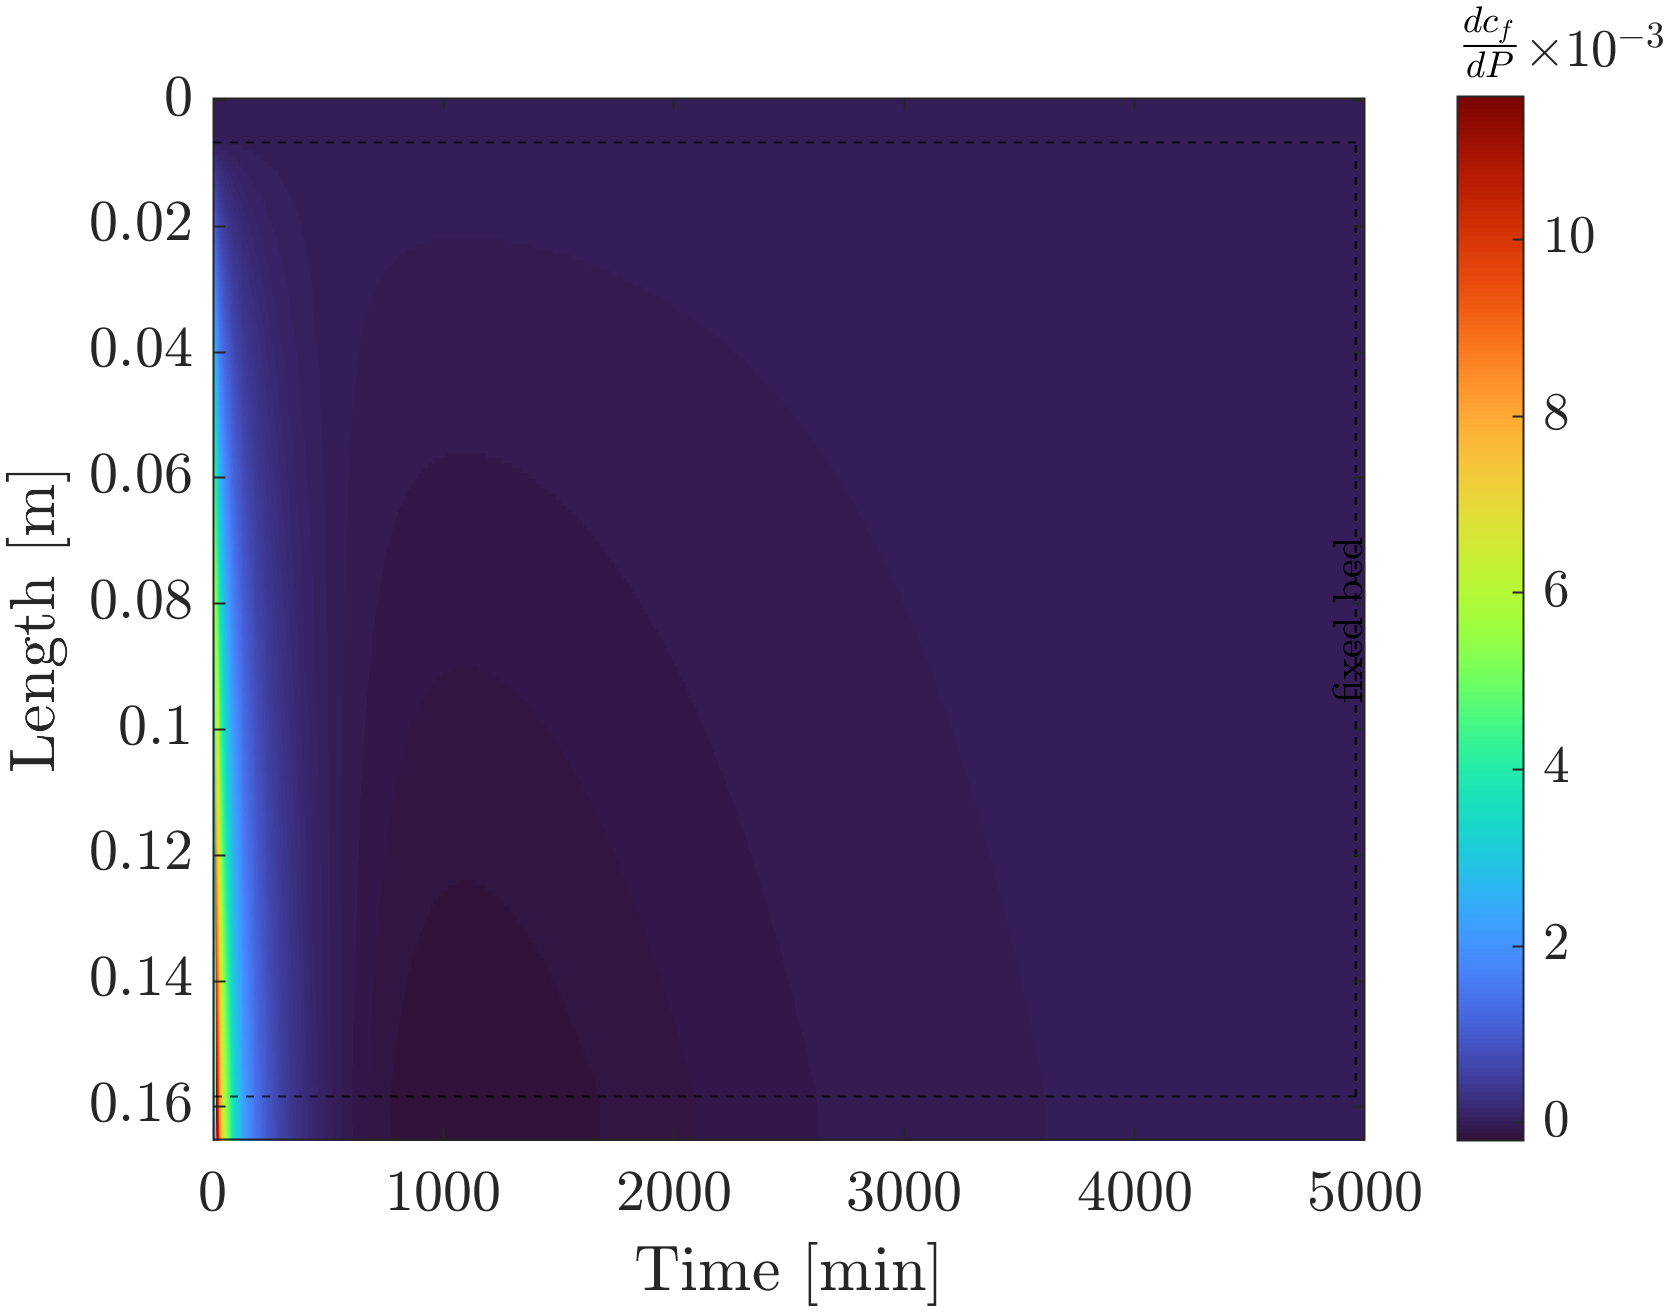
\includegraphics[trim = 0.0cm 0.0cm 0.0cm 0.0cm,clip,width=0.9\columnwidth]{/Results_sensitivity/CF_P.png}
		\caption{The effect of $P$ change on $C_f$}
		\label{fig:Sensitivty_P_CF}
	\end{figure}
	
	Figure \ref{fig:Sensitivty_P_y} illustrates how sensitive the extraction yield is to pressure change. Initially, the sensitivity curve stays almost flat, suggesting a latency in the system's response to pressure changes. A minor decrease in sensitivity arises due to a decrease in the velocity of the fluid phase. As the fluid moves slower, it reaches the end of the extractor later, which causes negative sensitivities.
	
	As the process continues and the solute reaches the extractor's outlet, the sensitivity curve increases rapidly, indicating an improvement in the process efficiency. This increase in sensitivity can be associated with the enhanced solubility and mass transfer imparted by higher pressures. The peak in $\frac{dy}{dP}$ reflects when the deviation from the original system is the largest.
	
	Beyond the peak, the sensitivity declines, converging towards zero. This descending curve represents a depletion phase: as the available solute in the solid phase diminishes, the potential for further increasing the yield through pressure alone is reduced. The remaining concentration gradient becomes a limiting factor, and the enhanced mass transfer no longer plays a dominant role compared to the original system.
	
	\begin{figure}[h!]
		\centering
		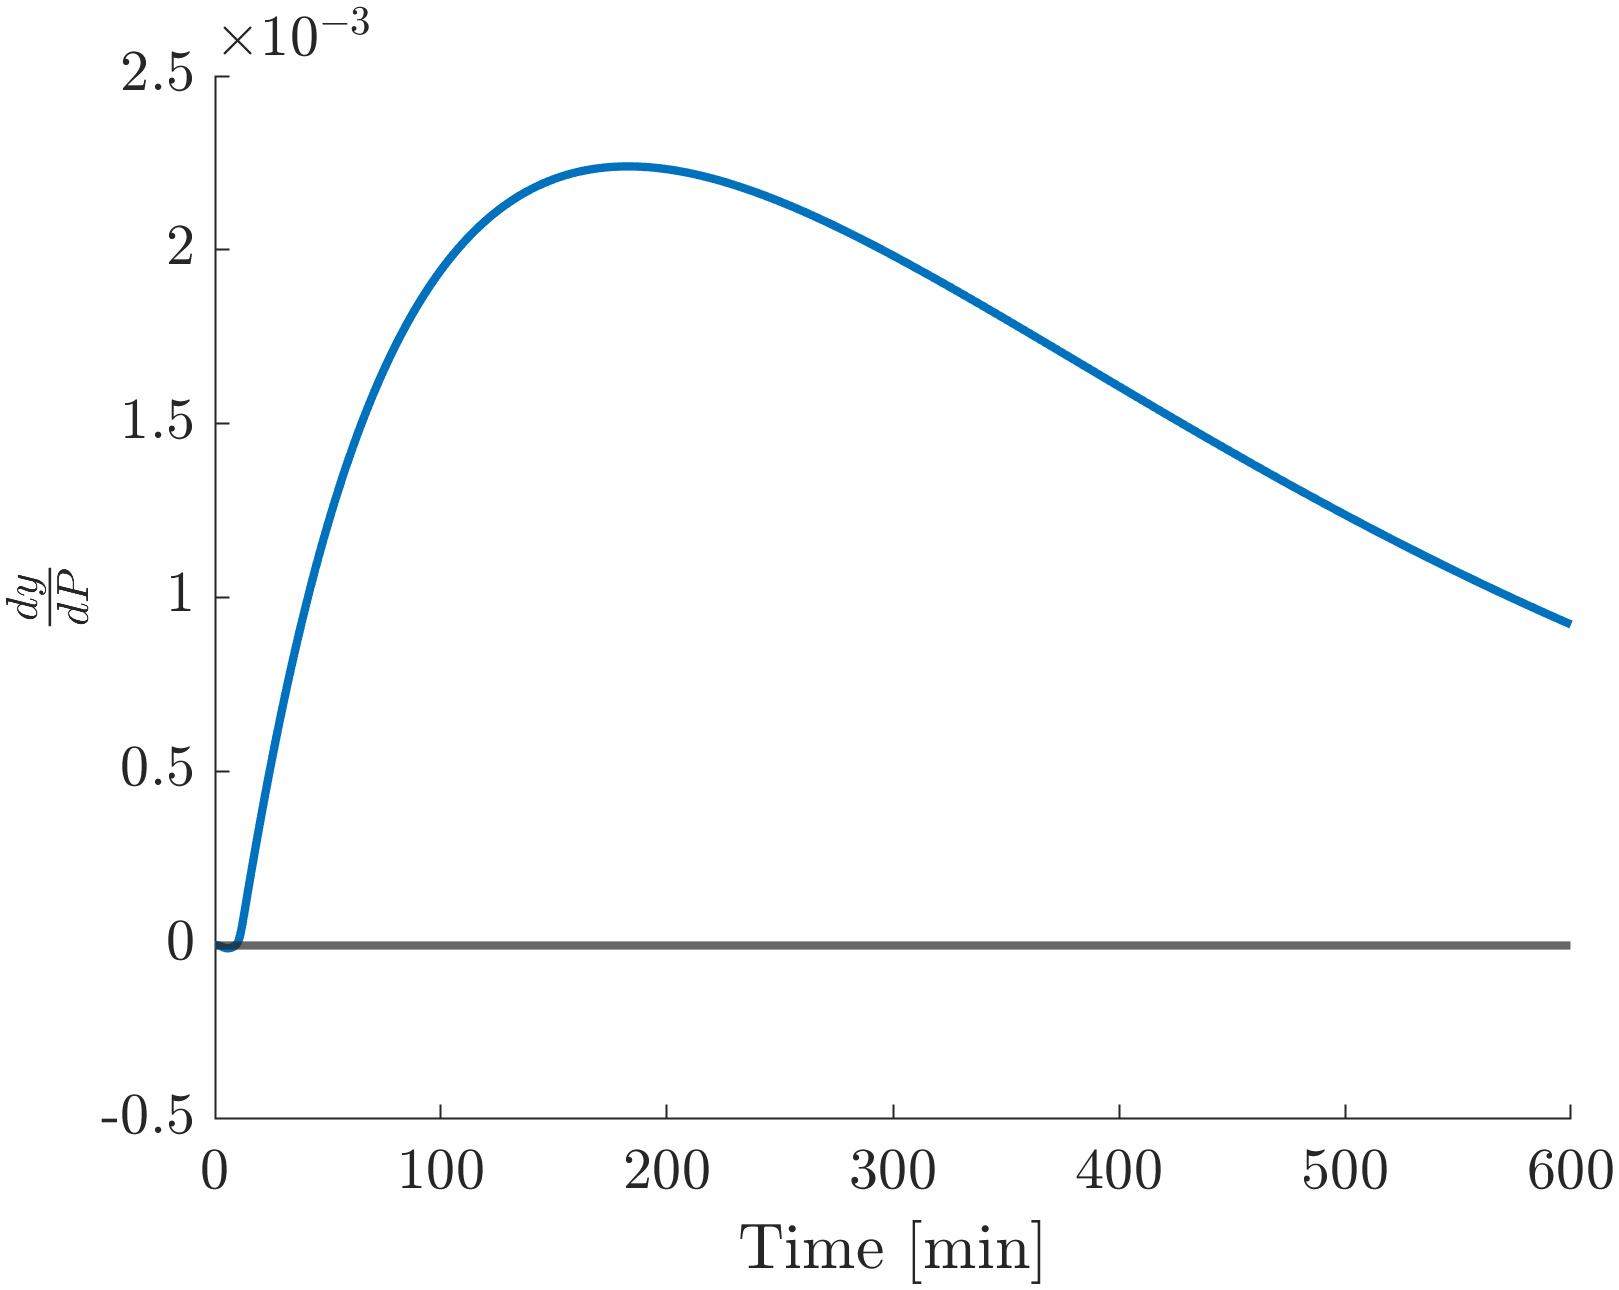
\includegraphics[trim = 0.0cm 0.0cm 0.0cm 0.0cm,clip,width=0.9\columnwidth]{/Results_sensitivity/Y_P.png}
		\caption{The effect of $P$ change on $y(t)$}
		\label{fig:Sensitivty_P_y}
	\end{figure}
		
\end{document}


































